%' Tree graph to explain the difference between partial-pooling and not
%' 
%' @src: The 2nd figure of the post 'Demystifying Item Response Theory (3/4)' 
%' @url: https://yongfu.name/2023/03/29/irt3/
\documentclass[preview,border=0]{standalone}
\usepackage[paperheight=20cm,paperwidth=15cm]{geometry}
\usepackage{graphicx}
\usepackage{amsmath}
\usepackage{tikz-qtree}
\usepackage{kmath,kerkis}

\begin{document}
\begin{center}

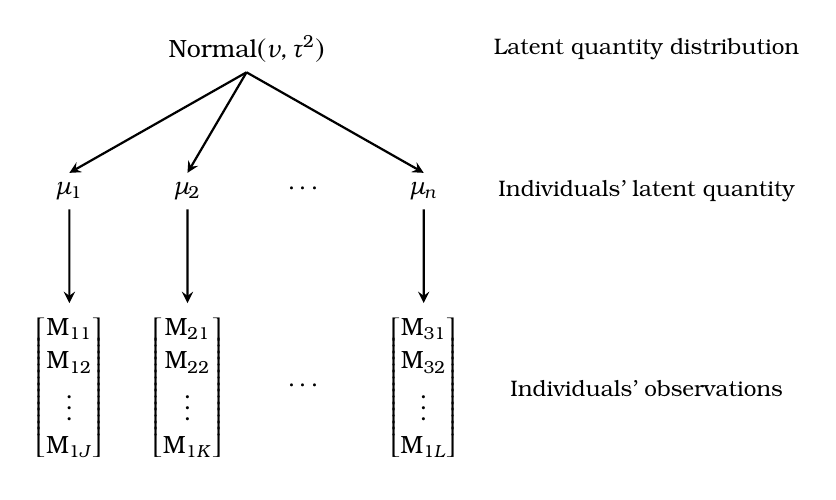
\begin{tikzpicture}[
    thick, % line style
    > = stealth, % arrow head style
    level distance=1.8cm,
    level 2/.style ={level distance=2.5cm},
    % level 1/.style={sibling distance=3.5cm},
    % level 2/.style={sibling distance=1cm},
    % level 3/.style={sibling distance=1cm}
]
% \tikzstyle{every edge}=[circle,draw]
\node (R) { $\text{Normal}(\nu, \tau^2)$ }
    child {node (a) {$\mu_1$} 
        child {
            node (b) { $\begin{bmatrix} \text{M}_{11} \\ \text{M}_{12} \\ \vdots \\ \text{M}_{1J} \end{bmatrix}$ } 
            edge from parent[->] }
        edge from parent[->] 
    }
    child {node {$\mu_2$} 
        child {
            node { $\begin{bmatrix} \text{M}_{21} \\ \text{M}_{22}  \\ \vdots \\ \text{M}_{1K} \end{bmatrix}$ } 
            edge from parent[->] }
        edge from parent[->] 
    }
    child {node {$\cdots$} 
        child {node {$\cdots$} edge from parent[draw=none] }
        edge from parent[draw=none] 
    }
    child {node {$\mu_n$} 
        child {
            node { $\begin{bmatrix} \text{M}_{31} \\ \text{M}_{32}  \\ \vdots \\ \text{M}_{1L} \end{bmatrix}$ } 
            edge from parent[->] }
        edge from parent[->] 
    };

    \path (R) ++(1.5in,0)coordinate(R0)  node [thick] { } ++(.5in,0)  node [] {\small Latent quantity distribution};
    \node at (a -| R0)(a0) { } (a0)++(.5in,0)  node [] {\small Individuals' latent quantity};
    \node at (b -| R0)(b0) { } (b0)++(.5in,0)  node [] {\small Individuals' observations};
\end{tikzpicture}


\end{center}
\end{document}